\documentclass[11pt a4paper]{article}
\usepackage[margin=2cm]{geometry}
\usepackage{amsmath, amssymb}
\usepackage{graphicx}
\usepackage{float}
\usepackage{aligned-overset}
\usepackage{subcaption}
\usepackage{tabularx} % fuer gleichungen nebeneinander
\usepackage{wrapfig} % damit figures neben text sien koennen

% partielle ableitungen
\newcommand{\delr}{\partial_r}
\newcommand{\delt}{\partial_t}
\newcommand{\deltheta}{\partial_\theta}
\newcommand{\delphi}{\partial_\varphi}

% elektrische feldkonstante
\newcommand{\epsz}{\epsilon_0}
% 1 / 4pi eps
\newcommand{\kco}{\frac{1}{4\pi\epsilon_0}}
% del fuer partial
\newcommand{\del}{\partial}

% div und rot
\newcommand{\diver}{\vec \nabla \cdot}
\newcommand{\rot}{\vec \nabla \times}
\newcommand{\grad}{\vec \nabla}

% hyperbolische funktionen
\newcommand{\arsinh}{\text{arsinh}}
\newcommand{\arcosh}{\text{arcosh}}
\newcommand{\artanh}{\text{artanh}}

% fuer impedanzen 
\newcommand{\omegaC}{\omega C}
\newcommand{\omegaL}{\omega L}
\newcommand{\omegaR}{\omega R}
\newcommand{\omegaLC}{\omega LC}
\newcommand{\omegaLCR}{\omega LCR}
\newcommand{\omegaCR}{\omega CR}

% fancy header
\usepackage{fancyhdr}
\fancyhf{}
% vspaces in den headern fuer Distanzen notwendig
% linke Seite: Namen der Abgabegruppe
\lhead{\textbf{Matthias Maile\\Roman Surma}\vspace{1.5cm}}
% rechte Seite: Modul, Gruppe, Semester
\rhead{\textbf{Physik II - Gruppe 2\\Sommersemester 2020}\vspace{1.5cm}}
% Center: nr. des blattes
\chead{\vspace{2.5cm}\huge{\textbf{22. Übungsblatt}}}
% benoetigt damit der eigentliche Text nicht in der Überschrift steckt
\setlength{\headheight}{4cm}

% zum zeichnen tikz
\usepackage{tikz}

% fuer fabigen text
\usepackage{xcolor}

% irgendwas mit figures
\usepackage{subcaption}

\begin{document}
\thispagestyle{fancy}

\begin{figure}[H]
	\centering
	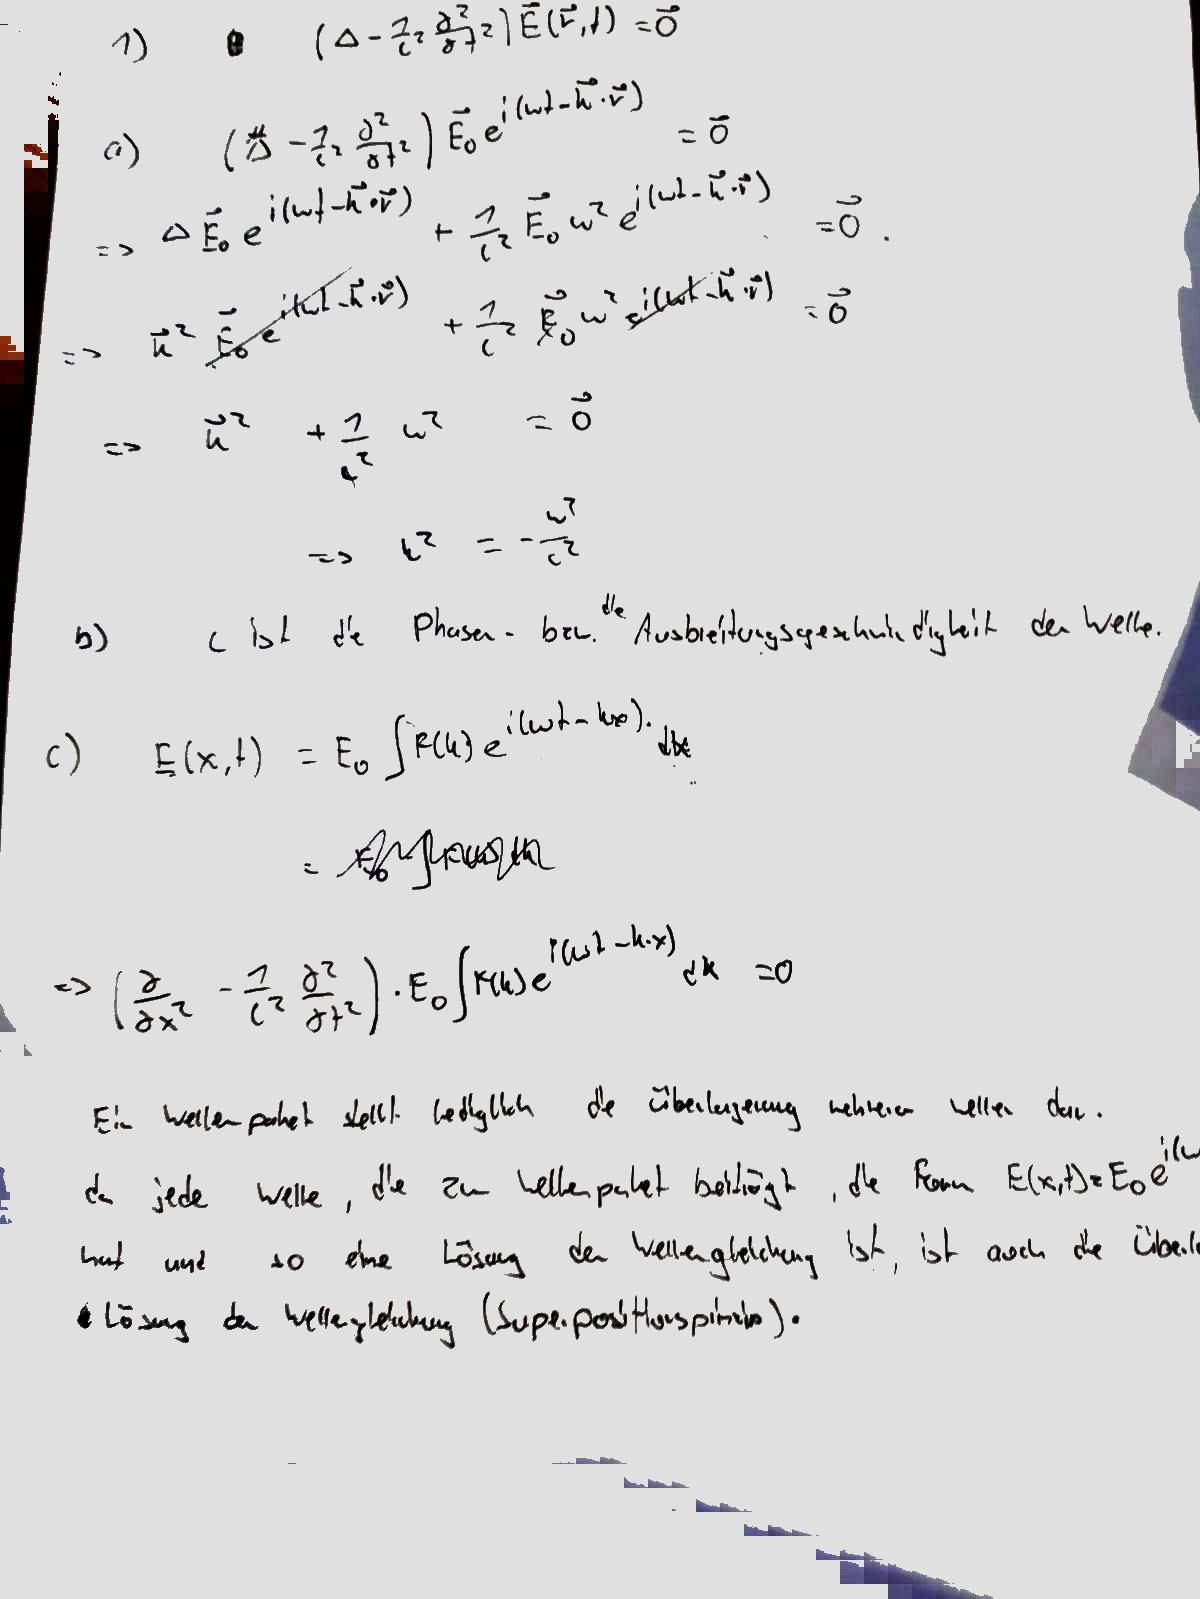
\includegraphics[width=15cm]{roman/1abc.jpg}
\end{figure}

\newpage
\setlength{\headheight}{0cm}

\begin{figure}[H]
	\centering
	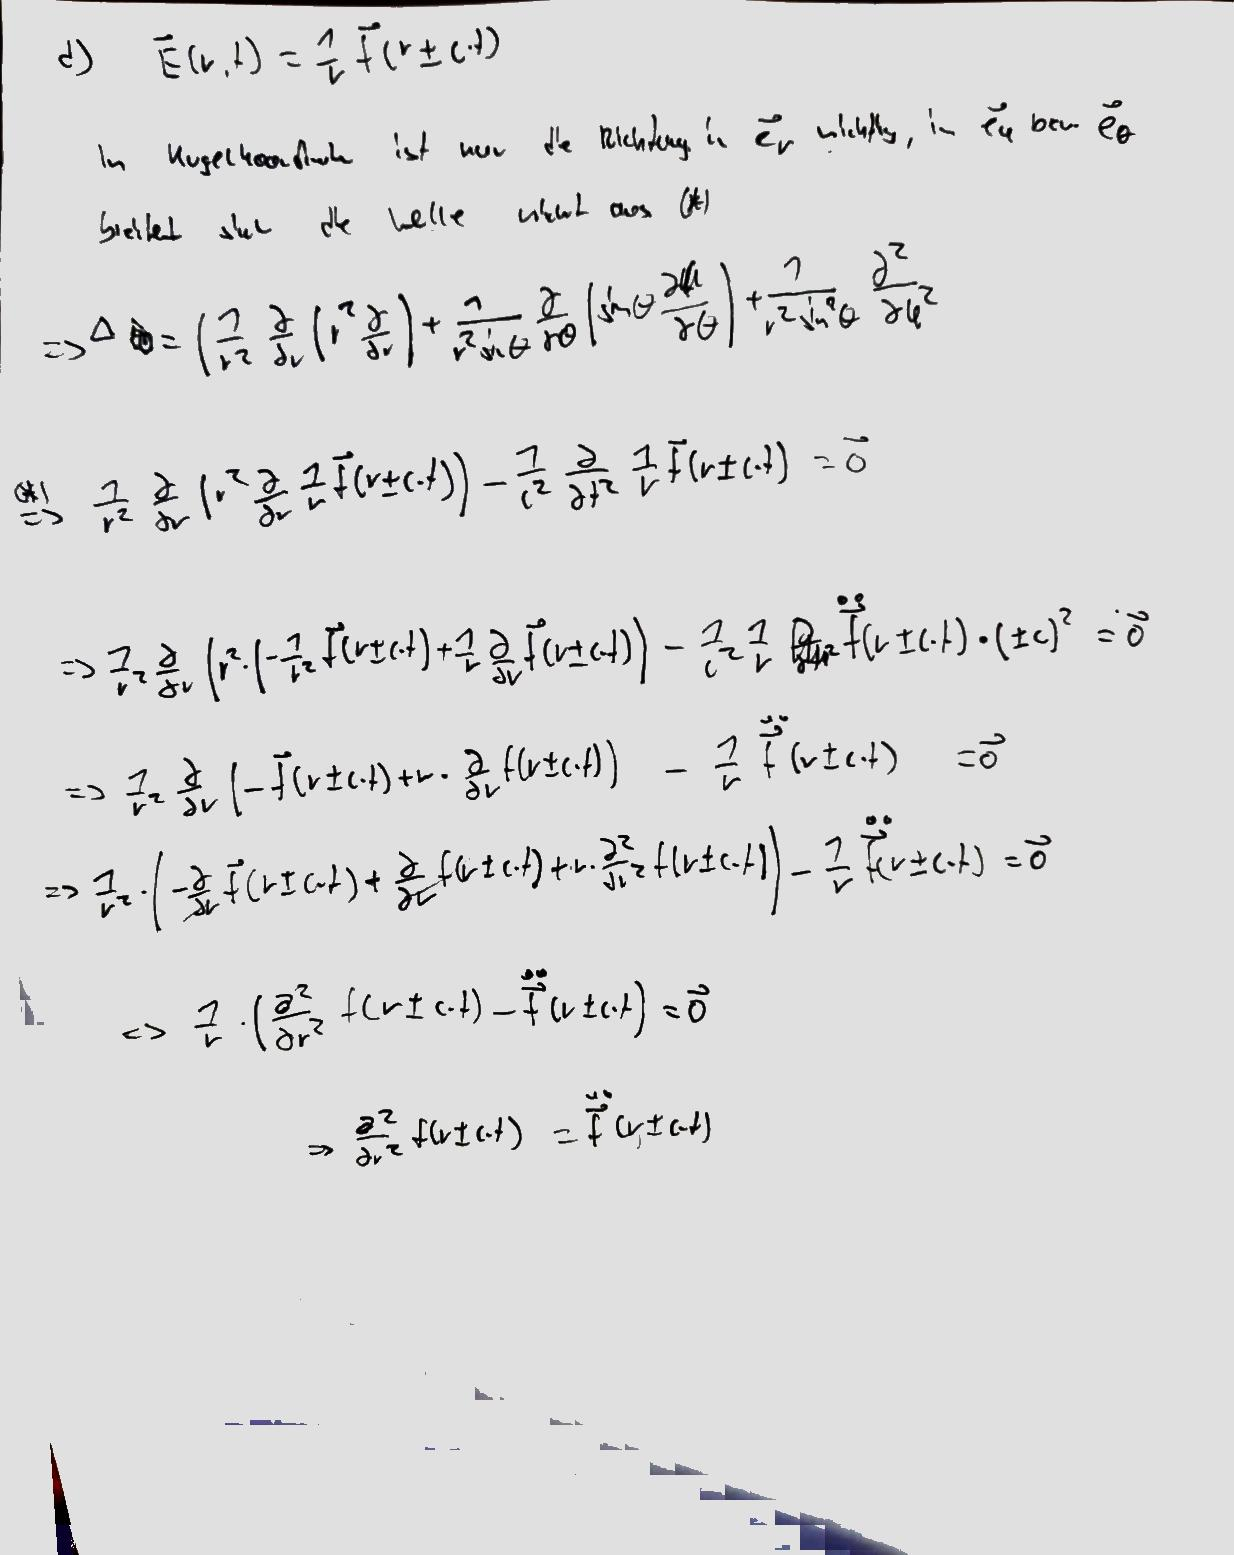
\includegraphics[width=15cm]{roman/1d.jpg}
\end{figure}

\newpage
\setlength{\headheight}{0cm}
\section*{Aufgabe 2}
a) Das Dipolmoment und seine Ableiutungen lauten:
\begin{align*}
	\vec p(t) 
	= \vec p_0 e^{-i\omega t}
	\qquad
	\dot{\vec p}(t) 
	= -i\omega \ \vec p_0 e^{-i\omega t}
	\qquad
	\ddot{\vec p}(t) 
	= -\omega^2 \ \vec p_0 e^{-i\omega t}
	\qquad \text{mit }
	\vec p_0 = p_0 \vec e_z
\end{align*}
Dann lässt sich für die Divergenz des Vektorpotentials zeigen:
\begin{align*}
	\diver \vec A(\vec r, t)
	&= \diver \frac{\mu_0}{4\pi r} \dot{\vec p} \left(t - \frac rc\right) \\
	% p einsetzen
	&= \diver \frac{-i \omega \mu_0}{4\pi r} \vec p_0 \exp \left( i\omega \frac rc - i\omega t \right) \\
	% divergenz nach vorne
	&= 
		\frac{-i \omega \mu_0}{4\pi}  \
		\diver \vec p_0 \frac{\exp\left(i\omega\frac rc - i\omega t\right)}{r} \\
	% produktregel
	&= 
		\frac{-i \omega \mu_0}{4\pi}  \
		\Bigg (
			\frac{\exp\left(i\omega\frac rc - i\omega t\right)}{r}  
			\underbrace{\diver \vec p_0}_{=0}
			+ \vec p_0 \cdot \vec \nabla \frac{\exp\left(i\omega\frac rc - i\omega t\right)}{r}
		\Bigg ) \\
	% 0 Term rausstriechen
	&= 
		\frac{-i \omega \mu_0}{4\pi}  \
		\Bigg (
			\vec p_0 \cdot \vec \nabla \frac{\exp\left(i\omega\frac rc - i\omega t\right)}{r}
		\Bigg ) \\
	% divergenz einsetze
	&= 
		\frac{-i \omega \mu_0}{4\pi}  \ \vec e_r \cdot \vec p_0 \cdot
		 \del_r \frac{\exp\left(i\omega\frac rc - i\omega t\right)}{r} \\
	% nach r ableiten
	&= 
		\frac{-i \omega \mu_0}{4\pi}  \ \vec e_r \cdot \vec p_0 \cdot
		 \frac{r 
		 	\frac{i\omega}{c} \exp\left(i\omega\frac rc - i\omega t\right)
		 	- \exp\left(i\omega\frac rc - i\omega t\right)}{r^2} \\
	% bruch trennen, r statt e_r
	&= 
		\frac{-i \omega \mu_0}{4\pi}  \ \vec r \cdot 
		\left(
		 \frac{\vec p_0 i\omega \exp\left(i\omega\frac rc - i\omega t\right)}{c r^2}
		 - \frac{\vec p_0 \exp\left(i\omega\frac rc - i\omega t\right)}{r^3}
		\right) \\
	% iomega reinziehen
	&= 
		- \frac{\mu_0}{4\pi}  \ \vec r \cdot 
		\Bigg(
		 \underbrace{\frac{-\omega^2 \vec p_0 \exp\left(i\omega\frac rc - i\omega t\right)}{c r^2}}
		 _{\frac{\ddot{\vec p}(t - r/c)}{cr^2}}
		 - \underbrace{\frac{i \omega \vec p_0 \exp\left(i\omega\frac rc - i\omega t\right)}{r^3}}
		 _{- \frac{\dot{\vec p}(t - r/c)}{r^3}}
		\Bigg) \\
	% p einsetzen
	&= 
		- \frac{\mu_0}{4\pi}  \ \vec r \cdot 
		\left(
			\frac{\ddot{\vec p} \left(t - \frac rc \right)}{cr^2} 
			+ \frac{\dot{\vec p}\left( t - \frac rc \right)}{r^3}
		\right) \\
	% epsz einsetzen
	&= 
		- \frac{\mu_0\epsz}{4\pi\epsz}  \ \vec r \cdot 
		\left(
			\frac{\ddot{\vec p} \left(t - \frac rc \right)}{cr^2} 
			+ \frac{\dot{\vec p}\left( t - \frac rc \right)}{r^3}
		\right) \\
	% nach c umstellen
	&= 
		- \frac{1}{c^2} \frac{1}{4\pi\epsz}  \ \vec r \cdot 
		\left(
			\frac{\ddot{\vec p} \left(t - \frac rc \right)}{cr^2} 
			+ \frac{\dot{\vec p}\left( t - \frac rc \right)}{r^3}
		\right) \\
	\overset{!}&{=} - \frac{1}{c^2} \dot \phi(\vec r, t) \\
	% nach dot phi uumstellen
	\Rightarrow \
	\dot \phi(\vec r, t)
	&= 
		\frac{1}{4\pi\epsz}  \ \vec r \cdot 
		\left(
			\frac{\ddot{\vec p} \left(t - \frac rc \right)}{cr^2} 
			+ \frac{\dot{\vec p}\left( t - \frac rc \right)}{r^3}
		\right) \\
	\Rightarrow \
	\phi(\vec r, t)
	&= 
		\frac{1}{4\pi\epsz}  \ \vec r \cdot 
		\left(
			\frac{\dot{\vec p} \left(t - \frac rc \right)}{cr^2} 
			+ \frac{\vec p\left( t - \frac rc \right)}{r^3}
		\right) + const.
\end{align*}

\newpage
b) Das $\vec E$-Feld in der Elektrodynamik ist gegeben durch 
\[ \vec E = -\grad \phi - \delt \vec A \]
Die zeitliche Ableitung von $\vec A$ lautet
\[ \delt A 
	= \delt \frac{\mu_0}{4\pi r} \dot{\vec p} \left(t - \frac rc\right) 
	= \frac{\mu_0}{4\pi r} \ddot{\vec p} \left(t - \frac rc\right) 
	= \frac{-\omega^2 \mu_0}{4\pi r} \vec p_0 \exp\left(\frac{i\omega r}{c} - i\omega t \right)
\]
aus $c = \frac{1}{\sqrt{\epsz \mu_0}}$ folgt, dass
\[ \delt A 
	= - \frac{1}{4\pi\epsz} \frac{\omega^2}{c^2 r} \vec p_0 \exp\left(\frac{i\omega r}{c} - i\omega t \right)
	\tag{2.1}
\]
Für $\grad \phi$ lässt sich schreiben:
\begin{align*}
	\grad \phi
	&= \grad
		\frac{1}{4\pi\epsz}  \ \vec r \cdot 
		\left(
			\frac{\dot{\vec p} \left(t - \frac rc \right)}{cr^2} 
			+ \frac{\vec p\left( t - \frac rc \right)}{r^3}
		\right) \\
	% umschreiben in e funktion
	&= \grad
		\frac{1}{4\pi\epsz}  \
		\underbrace{(\vec e_r \cdot \vec p_0)}_{p_0 \cos\theta} \
		\underbrace{\left(
			\frac{\exp\left(\frac{i\omega r}{c} - i\omega t \right)}{r^2}
			-
			\frac{i\omega \exp\left(\frac{i\omega r}{c} - i\omega t \right)}{cr}
		\right)}_{\alpha :=} \\
	&= \grad
		\frac{1}{4\pi\epsz} \ p_0 \cos\theta \cdot  \alpha \\
	% definiton des gradienten einsetzen
	&= \kco \Big( 
	\vec e_r \delr \left(p_0 \cos\theta \cdot \alpha \right) +
	\frac{\vec e_\theta}{r} \del_\theta \left(p_0 \cos\theta \cdot \alpha \right)
	+ \frac{\vec e_\phi}{r\sin\theta} 
	\underbrace{\del_\phi \left(p_0 \cos\theta \cdot \alpha \right)}_{0}
	\Big) \\
	% ableitungen richtig setzen
	&= \frac{p_0}{4\pi\epsz} \left(
		\vec e_r \cdot \cos\theta \cdot \delr\alpha 
		+
		\frac{\vec e_\theta \cdot \alpha}{r} \del_\theta \cos\theta
	\right)
\end{align*}
Die Nebenrechnung für $\delr \alpha$:
\begin{align*}
	\delr \alpha 
	&= \delr \left(\exp\left(\frac{i\omega r}{c} - i\omega t \right) \cdot
		\left(\frac{1}{r^2} - \frac{i\omega}{cr} \right)
	\right) \\
	&= 
		\exp\left(\frac{i\omega r}{c} - i\omega t \right) 
		\cdot \left(\frac{2i\omega}{cr^2} + \frac{\omega^2}{c^2r} -\frac{2}{r^3} \right)
\end{align*}
% einsetzen der Nebenrechnung in Hauptrechnung
\begin{align*}
	\Rightarrow
	\grad \phi
	&= \frac{p_0}{4\pi\epsz} \exp(\hdots)
	\left(
		\vec e_r \cdot \cos\theta \cdot 
		\left(\frac{2i\omega}{cr^2} + \frac{\omega^2}{c^2r} -\frac{2}{r^3} \right)
		+
		\vec e_\theta \cdot \sin\theta \cdot \left(\frac{1}{r^3} - \frac{i\omega}{cr^2} \right)
	\right)
\end{align*}
Mit der Eigenschaft $\vec e_z = \vec e_r \cos\theta - \vec e_\theta \sin\theta$ lässt sich der 
Ausdruck (2.1) für $\delt \vec A$ umschreiben:
\begin{align*}
	\delt \vec A
	&= - \frac{1}{4\pi\epsz} \ \frac{\omega^2}{c^2 r} \ 
	\vec p_0 \exp\left(\frac{i\omega r}{c} - i\omega t \right) \\
	% \vec p_0 umschreiben
	&= - \frac{1}{4\pi\epsz} \ \frac{\omega^2}{c^2 r} \ 
	p_0 \cdot \vec e_z \exp\left(\frac{i\omega r}{c} - i\omega t \right) \\
	&= \frac{p_0}{4\pi\epsz} \
	\exp(\hdots)  \
	\frac{\omega^2}{c^2 r} 
	\left(\vec e_\theta \sin\theta - \vec e_r \cos\theta \right)
	\\
\end{align*}

\newpage
Dann lauten die Kompenenten des $\vec E$-Feldes:
\begin{align*}
	% r richtung
	E_r 
	&= -\left(\grad \phi \right)_r -\left(\delt \vec A \right)_r  \\
	&= - \frac{p_0}{4\pi\epsz} \exp\left(\frac{i\omega r}{c} - i\omega t \right) \cdot \cos\theta
	\cdot \left(\frac{2i\omega}{cr^2} + \frac{\omega^2}{c^2r} -\frac{2}{r^3} - \frac{\omega^2}{c^2r} \right) \\
	% kuerzen
	&= \frac{p_0}{2\pi\epsz} \exp\left(\frac{i\omega r}{c} - i\omega t \right) \cdot \cos\theta
	\cdot \left(\frac{1}{r^3} - \frac{i\omega}{cr^2} \right) \\
	% theta richtung
	E_\theta
	&= -\left(\grad \phi \right)_\theta -\left(\delt \vec A \right)_\theta  \\
	&= - \frac{p_0}{4\pi\epsz} \exp\left(\frac{i\omega r}{c} - i\omega t \right) \cdot \sin\theta
	\cdot \left(\frac{\omega^2}{c^2r} - \frac{i\omega}{cr^2} + \frac{1}{r^3} \right)
\end{align*}
\begin{figure}[H]
	\centering
	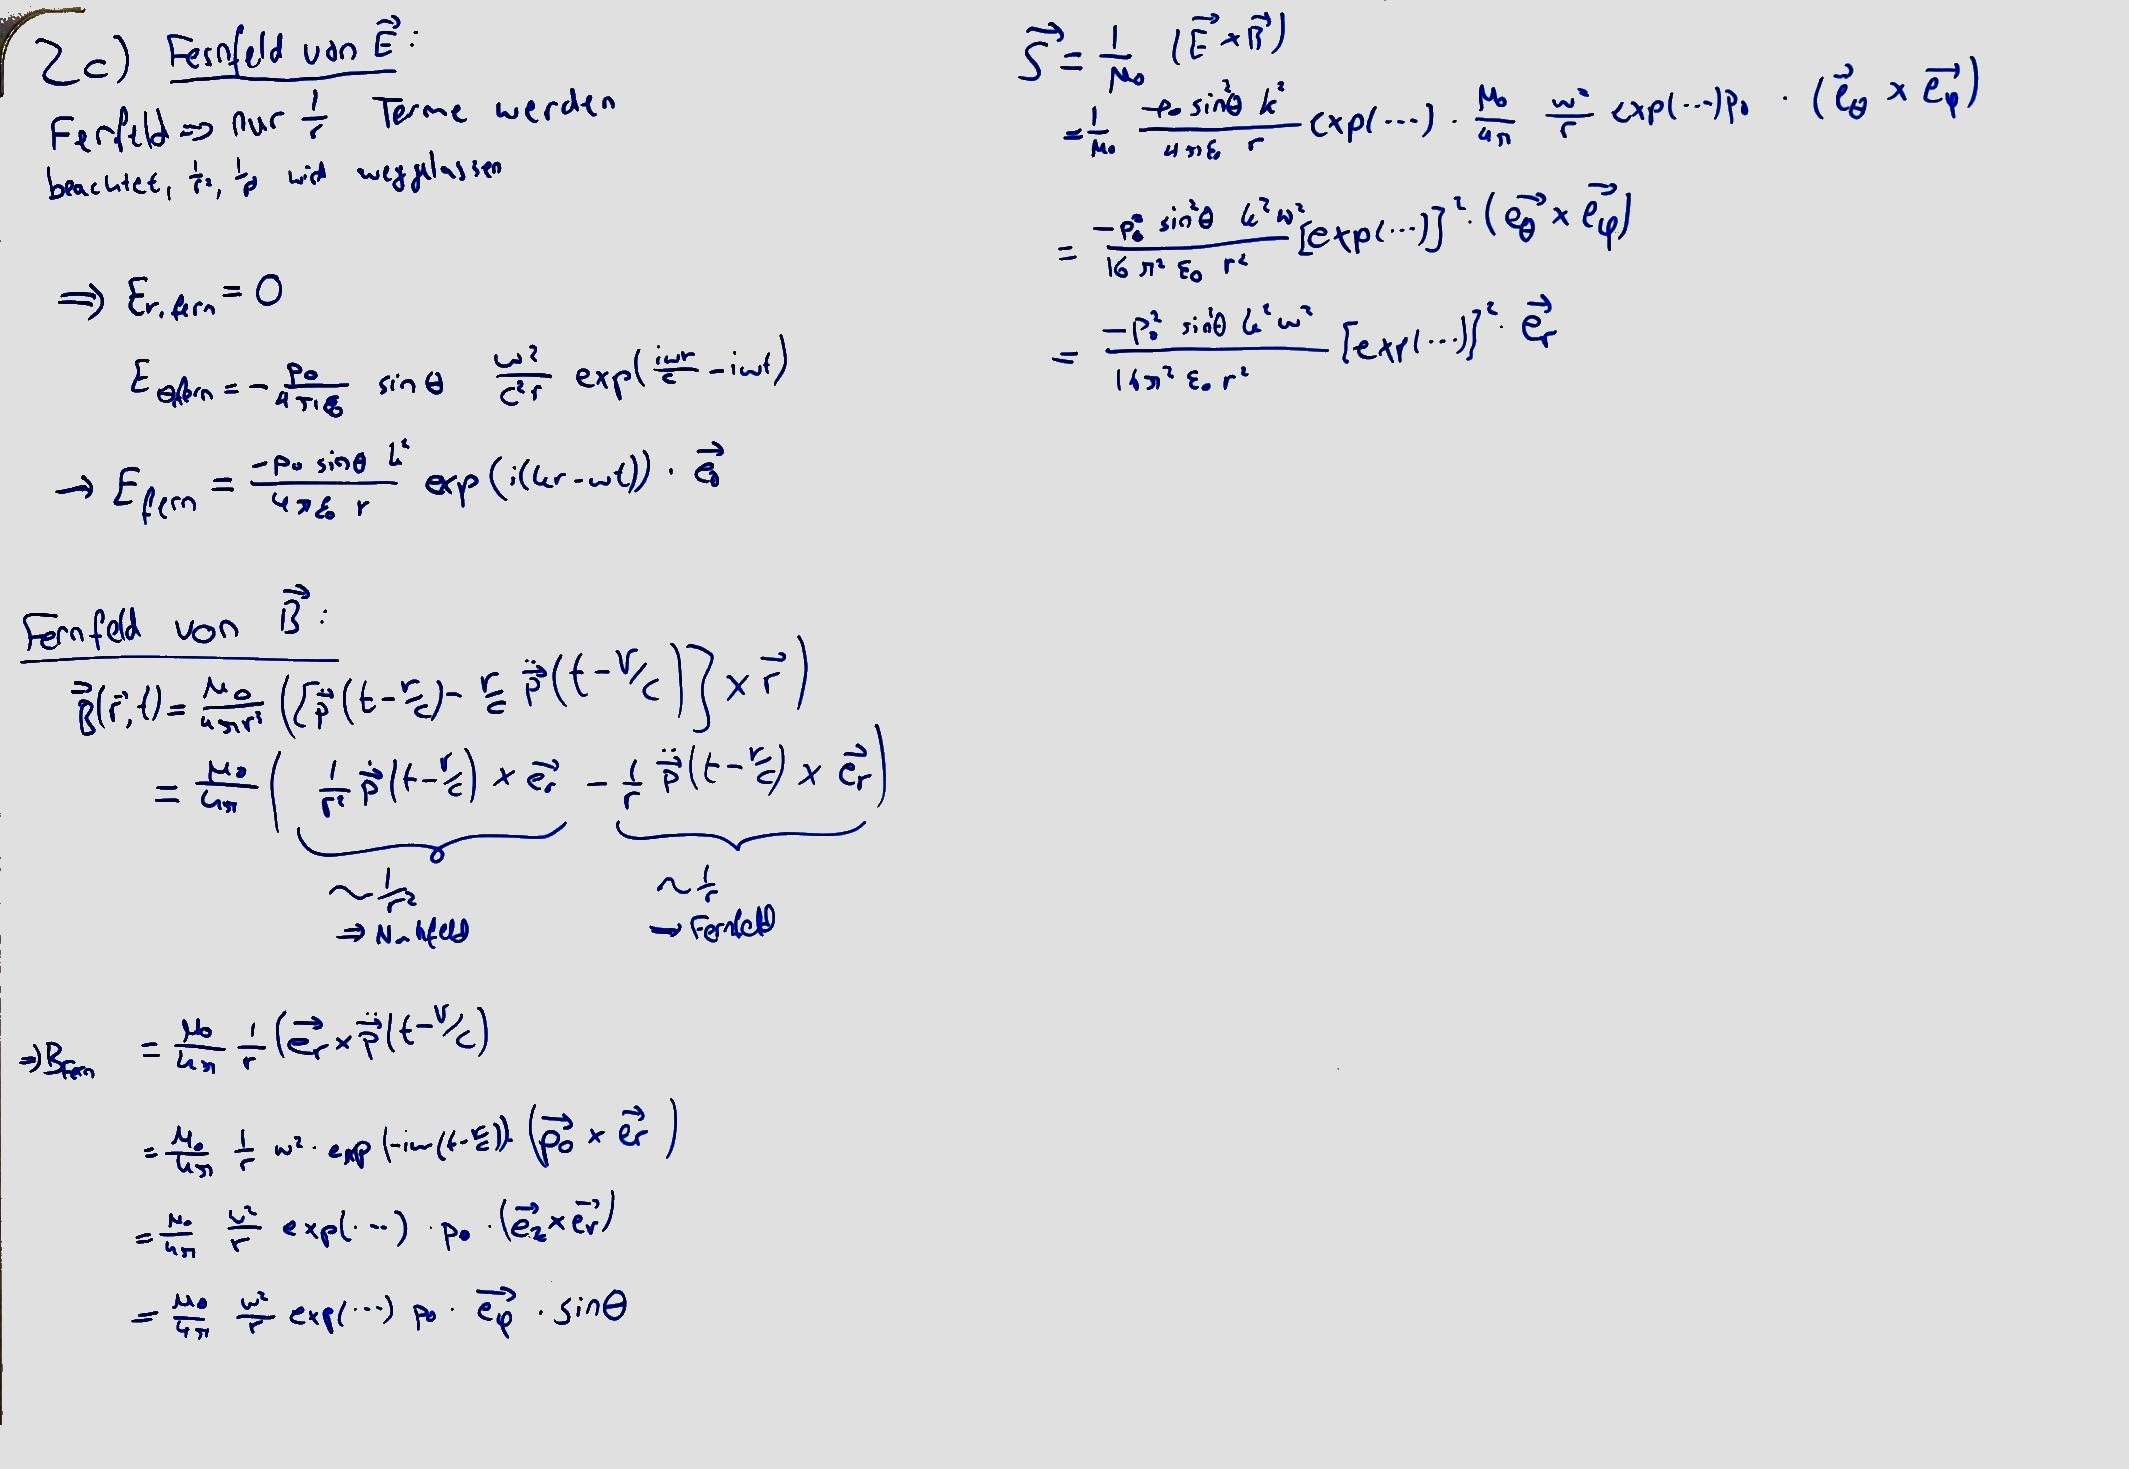
\includegraphics[width=17cm]{2c.jpg}
\end{figure}
Der Ponynting Vektor zeigt (aufgrund des negativen Vorzeichens in der Rechnung, wahrscheinlich irgendwo eins 
falsch gesetzt) vom Beobachter zur Quelle.
\[ \vec S \parallel \vec e_r \]
Auf der Äquatorialebene ist dieser am stärksten, bei den Polen geht dieser gegen 0.

\newpage

\begin{figure}[H]
	\centering
	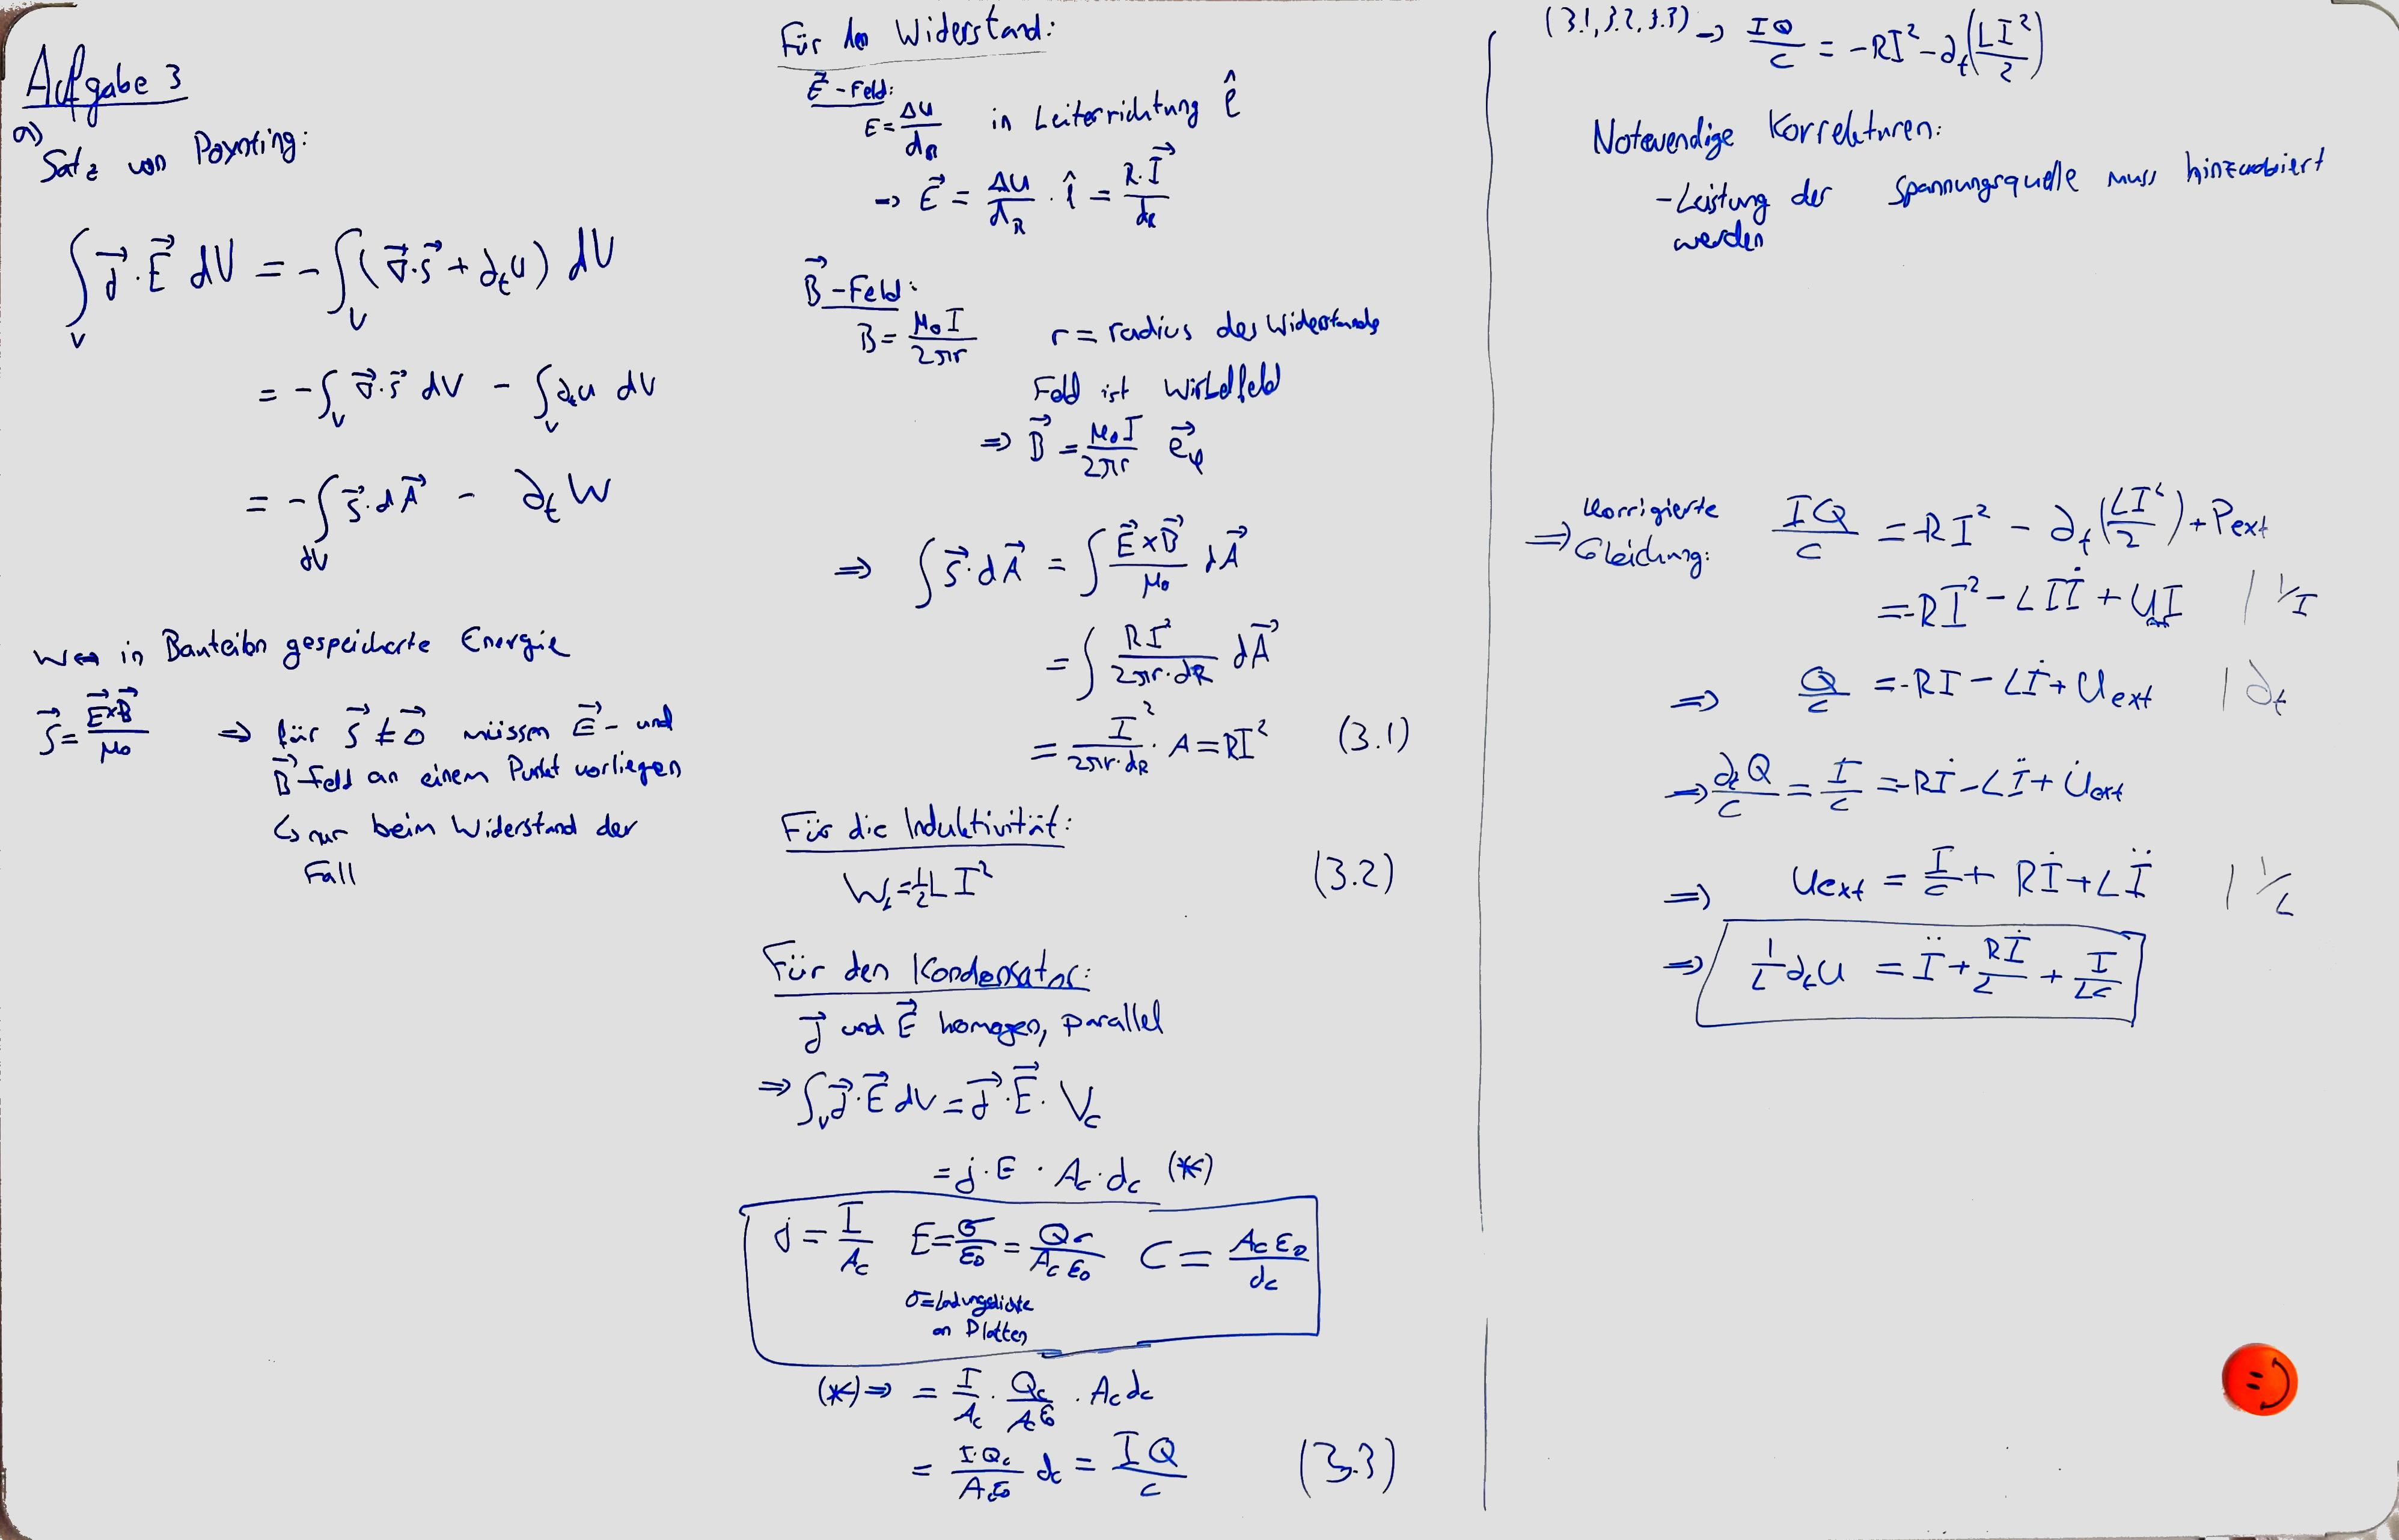
\includegraphics[width=18cm]{3a.jpg}
\end{figure}

\begin{wrapfigure}{l}{0.5\textwidth}
	\centering
	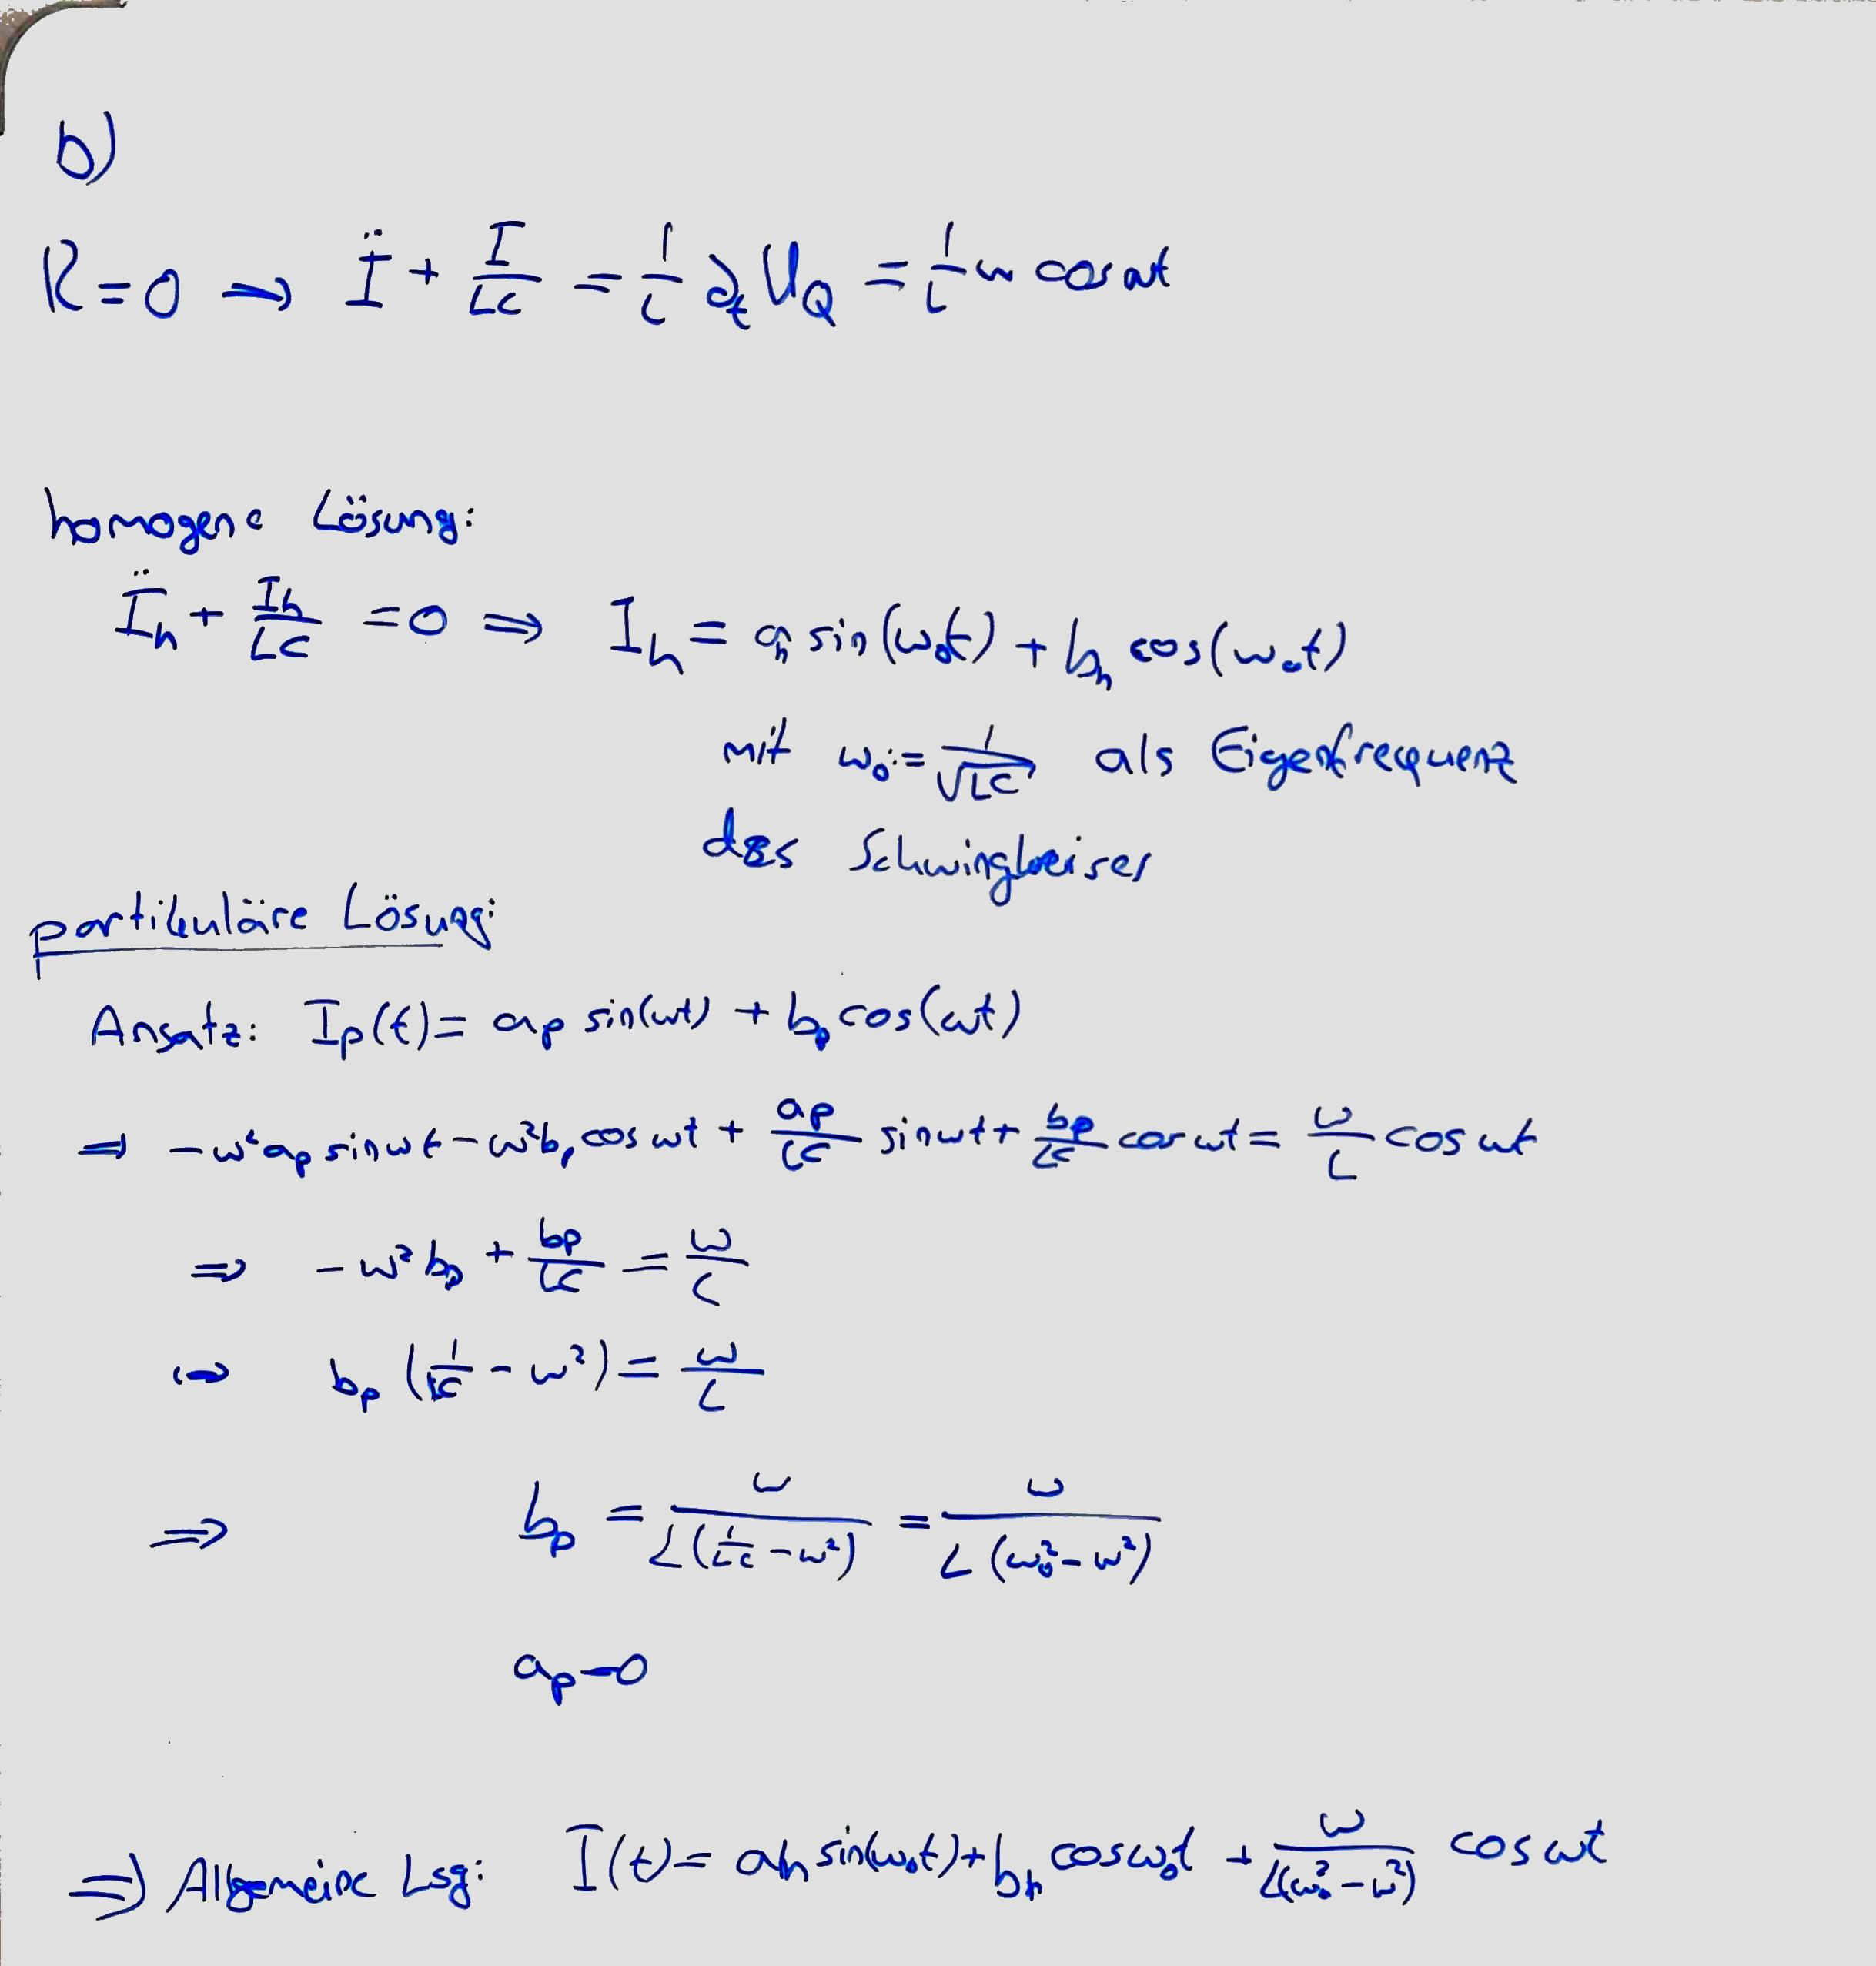
\includegraphics[width=8cm]{3b.jpg}
\end{wrapfigure}
Für $\omega$: \\
Die Anrgefrequenz $\omega$ sollte von der Eigenfrequenz $\omega_0$ des Schwingkreises abweichen, da es sonst 
zu einer Resonanzkatastrophe kommen kann (in der Gleichung einem durch 0 teilen entsprechend). \\
Da in der Realität zumindest durch die Bauteile immer eine geringe Dämpfung stattfindet gäbe es ein 
``Maximum`` für die Resonanz. \\
Da es aber dennoch zu Schäden durch zu hohen Stromfluss kommen kann, sollte dies bei Schaltungen beachtet werden.

\newpage

\begin{figure}[H]
	\centering
	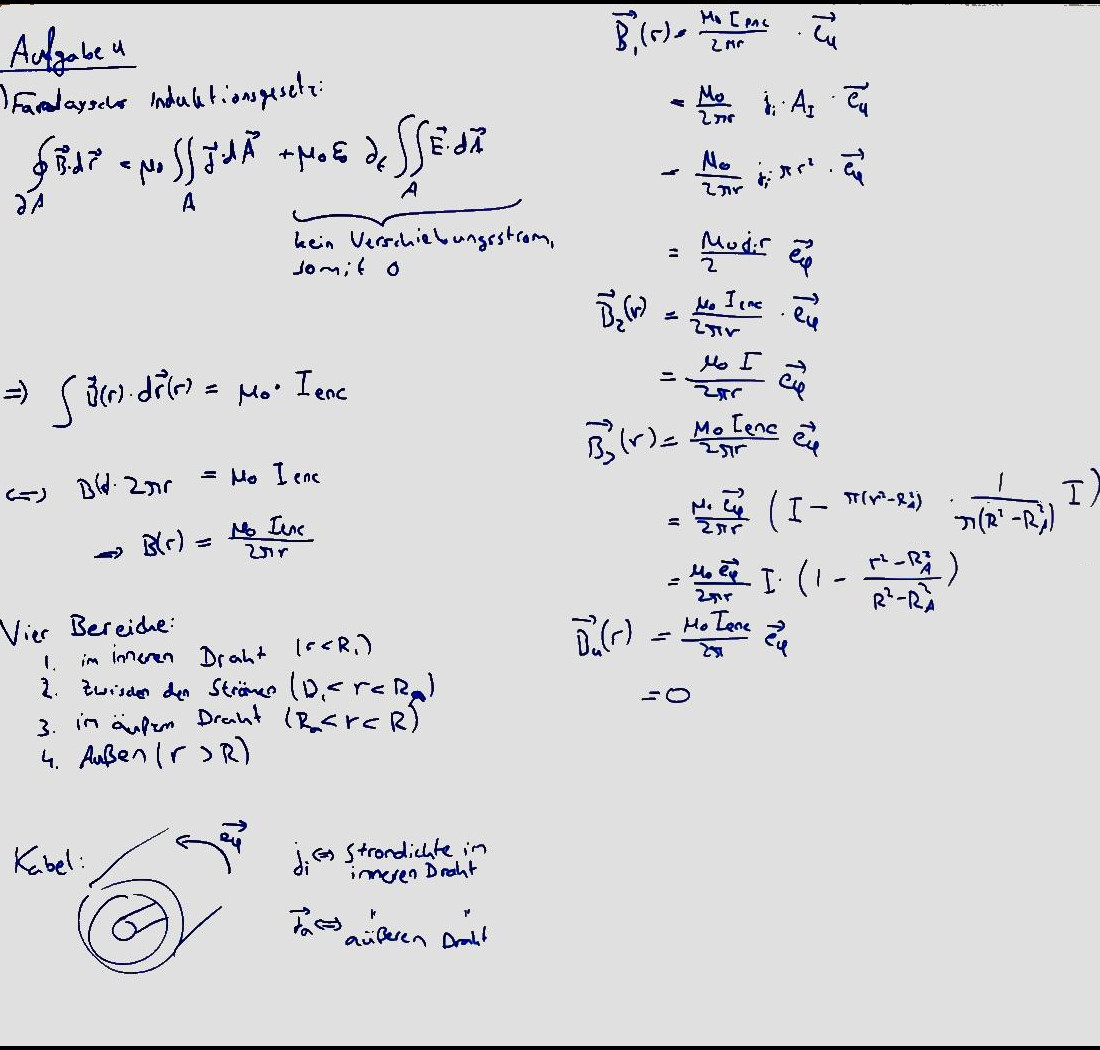
\includegraphics[width=18cm]{4a.jpg}
\end{figure}

\begin{figure}[H]
	\centering
	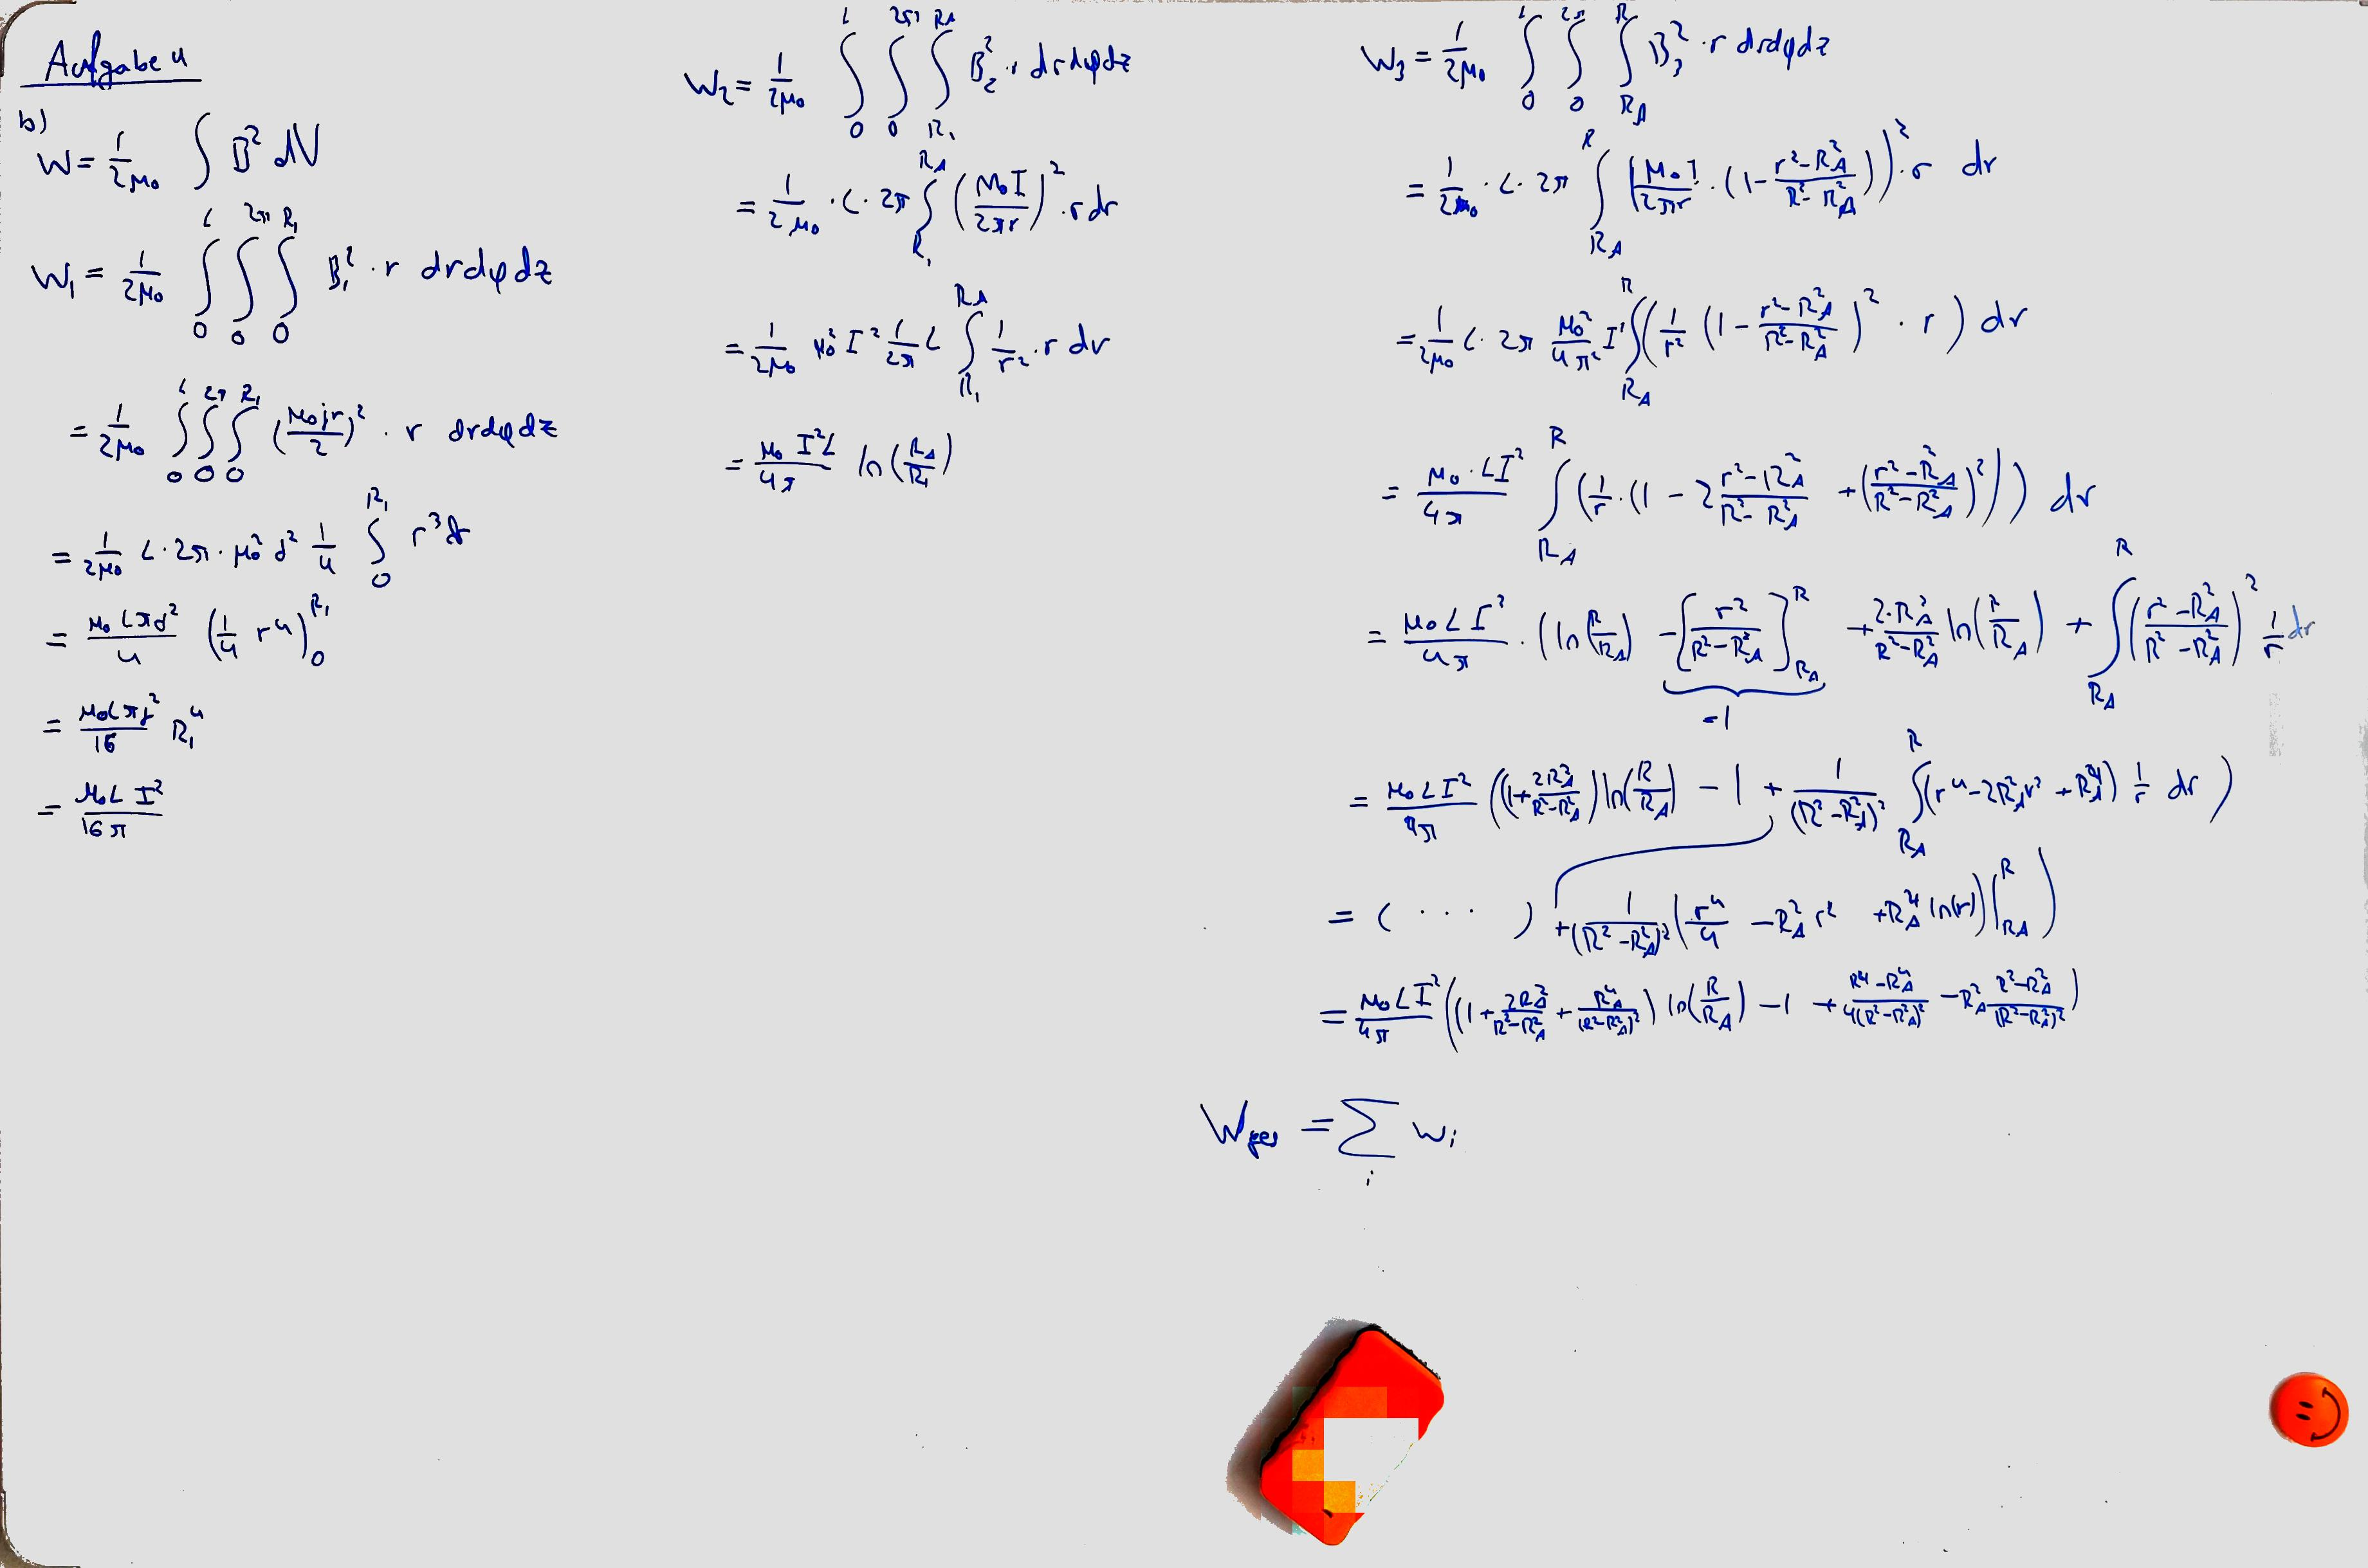
\includegraphics[width=18cm]{4b.jpg}
\end{figure}

c) Ein Vorteil des Koaxialkabels ist die verbessert Abschirmung gegen externe Magnetfelder, bzw. dass andere
Kabel in der Umgebung von diesem kein Magnetfeld erfahren.

\end{document}
